\documentclass[tikz,border=7pt]{standalone}
\usepackage{amsmath}
\usetikzlibrary{arrows.meta,positioning}

\definecolor{ink}{HTML}{21352F}
\definecolor{teal}{HTML}{087F7B}
\definecolor{rose}{HTML}{B65A62}
\definecolor{gold}{HTML}{C58B2A}
\definecolor{blue}{HTML}{4B77A8}

\begin{document}
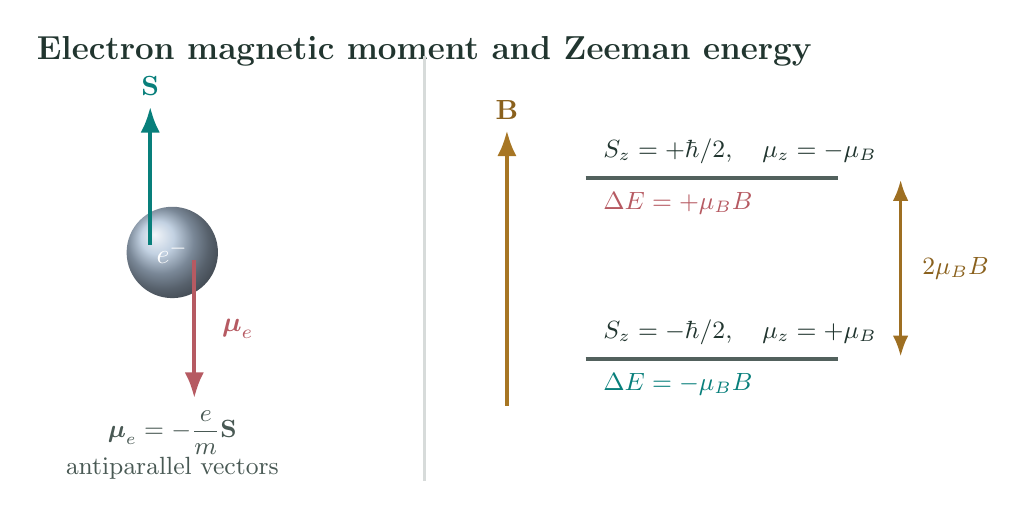
\begin{tikzpicture}[
  font=\sffamily,
  >=Latex,
  vector/.style={->,line width=1.4pt},
  level/.style={line width=1.4pt,draw=ink!78}
]
  \node[font=\bfseries\large,text=ink] at (0,2.75)
    {Electron magnetic moment and Zeeman energy};

  \shade[ball color=blue!45] (-3.2,0.2) circle (0.58);
  \node[font=\bfseries,text=white] at (-3.2,0.2) {$e^-$};

  \draw[vector,teal] (-3.48,0.3) -- (-3.48,2.05)
    node[above,text=teal,font=\bfseries] {$\mathbf S$};
  \draw[vector,rose] (-2.92,0.1) -- (-2.92,-1.65)
    node[midway,right=6pt,text=rose,font=\bfseries]
    {$\boldsymbol\mu_e$};

  \node[align=center,text=ink!82,font=\small] at (-3.2,-2.25)
    {$\displaystyle \boldsymbol\mu_e=-\frac{e}{m}\mathbf S$\\
     antiparallel vectors};

  \draw[ink!18,line width=1pt] (0,-2.7) -- (0,2.7);

  \draw[vector,gold!85!black] (1.05,-1.75) -- (1.05,1.75)
    node[above,text=gold!70!black,font=\bfseries] {$\mathbf B$};

  \draw[level] (2.05,1.15) -- (5.25,1.15);
  \node[anchor=west,text=ink,font=\small] at (2.15,1.48)
    {$S_z=+\hbar/2,\quad \mu_z=-\mu_B$};
  \node[anchor=west,text=rose,font=\small] at (2.15,0.82)
    {$\Delta E=+\mu_BB$};

  \draw[level] (2.05,-1.15) -- (5.25,-1.15);
  \node[anchor=west,text=ink,font=\small] at (2.15,-0.82)
    {$S_z=-\hbar/2,\quad \mu_z=+\mu_B$};
  \node[anchor=west,text=teal,font=\small] at (2.15,-1.48)
    {$\Delta E=-\mu_BB$};

  \draw[<->,draw=gold!80!black,line width=1pt]
    (6.05,-1.12) -- (6.05,1.12)
    node[midway,right=4pt,text=gold!70!black,font=\small]
    {$2\mu_BB$};
\end{tikzpicture}
\end{document}
